\section{LSTM Method}
The lstm...

% Train val split
%When working with time series it is important to think about how one splits up
%the dataset into training, validation, and test set.
%One key aspect when forecasting a time series is the newer the information,
%the more relevant it is for the forecast.
%In a perfect world the model will be able to use all the available data for training,
%right up to the point of forecast, then try to forecast the wanted horizon.
%However, in order to tune hyperparameters and avoid overfitting to the training
%set, we need a validation set.

In a stateful LSTM everything fed through the network is seen by the network
as follow each other in time. Since the validation step is executed at the end of
each epoch, and each epoch pass feeds all the training data through the network,
it makes sense to use the last section of the training data as the validation data.

The inspiration of the trainining, validation and test splitting is taken from
\cite{Bandara2019}, \cite{Hewamalage2021}.
Both are using competition datasets, in which the test data are already
removed from the training data.
\cite{Bandara2019} reserves the last $m$ sized part for validation from the training data,
where $m$ is the forecasting window size.... This means L - 2*(n+ m)
\cite{Hewamalage2021} reserves the last $m$ sized part for validation,
where $m$ is the forecasting window size.
But they point out that this is problematic becouse the last part of the sequence is
not considered for training the model.
The further away the test predictions are from the training set the worse,
because the underlying patterns may change during this last part of the sequence.
Therefore \cite{Hewamalage2021} will split the dataset during tuning, but when testing
they will train on all the available training data.

We made some modifications of \cite{Hewamalage2021} data split solution.
First, we have the complete datasets available, so we had to split out our
test set manually. Our test set from each time series consist of the last $m$ sized
sequence for forecasting.

Second, we used a stateful LSTM, which restricted the validation set to have the
same batch size as the training set. This meant that having a validation set equal
to the size of the forecast window $m$ would limit the batch size of the training set
to use a batch size equal to $m$. \cite{Bandara2019} would always
train their models on multiple time series, which meant that their validation set would
be $validation\_size = m * number\_of\_series$. In contrast we would also train models on
a single time series. In this case the validation set would be equal to one forecasting window.
When the forecasting window was of size 7 we found that this validation set got too small.
We experienced a wide range of optimal hyperparameters. These models did not seem to
learn anything meaninfule patterns from the training data, but would in most cases guess
the median.

As a result of the findings above we chose a batch size for the training set first, then
used the chosen batch size as a validation size.
This solution means that we cannot do a hyperparameter search for an optimal batch size
because that would change the validation set as well. When we tried this, the model would
almost always prefere the smallest possible batch size because that meant it would get a
small validation set, which also meant fewer possible errors it could make.

Same as \cite[]{Hewamalage2021} we would also split the training set into validation set for
hyperparameter tuning, but for testing we would train on the validation set as well.

%part L - (IW + OW) as test set,
%and the next part for validation L - 2(IW + OW) during tuning.
%But for testing and prediction they will train on the validation set as well
%because the last part of the sequence is not considered for training the model.
%The further away the test predictions are frin the training set, the worse
%because the underlying patterns may change during this last part of the sequence.


\begin{figure}[h!]
  \centering
  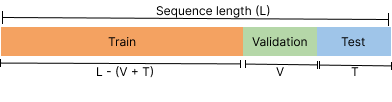
\includegraphics[width=0.7\textwidth]{./figs/illustrations/illustration_train_val_test_split.png}
  \hfill
  \caption{Illustration of trainig, validation, and test split. V = batch size, T = m = forecast window}
  \label{fig:train-val-test-split}
\end{figure}

\Cref{fig:train-val-test-split} shows an illustration of how one dataset is split up during
hyperparameter tuning.
The whole time series has a size of length $L$. The test set $T$ is taken from the end of the series,
and has the size of the forecast window $L = m$. The validation set $V$ has the size of
one batch size $V=batch\_size$. So during tuning the size of the training data is
$T = L - (V + T)$. During testing the validation set $V$ is re-added to the training set,
making the training set $T = L - T$.

\begin{figure}[h!]
  \centering
  
\includegraphics[width=0.7\textwidth]{./figs/illustrations/illustration_global_time_series.png}
  \hfill
  \caption{Illustration of how multiple time series are concatonated for the global method}
  \label{fig:global-time-series}
\end{figure}



% Tuning: How did we specify tuning ranges

% Model choice: 

% Hvordan har vi valgt å tune med trening og test set

% Global model, how did we train on multiple dataset?